\documentclass[11pt,a4paper]{article}
\usepackage[margin=1in]{geometry}
\usepackage{graphicx,booktabs,array,pdflscape,caption,hyperref,xcolor}
\usepackage[T1]{fontenc}
\hypersetup{colorlinks=true,linkcolor=blue!55!black,urlcolor=blue!55!black}
\captionsetup{font=small,labelfont=bf}
\setlength{\parskip}{0.35em}
\setlength{\parindent}{0pt}
\newcommand{\IRR}{\mathrm{IRR}}

\title{Forest Cover and Recorded CPI-Maoist Violence in India\\
\large A district-level descriptive analysis, 2001 forest cover and 2005--2025 events}
\author{Nakshatra Ghosh}
\date{30 September 2026}

\begin{document}
\maketitle

\begin{abstract}
This report examines whether districts with more pre-period forest cover recorded more CPI-Maoist violence. Forest Survey of India (FSI) 2001 forest statistics are linked to UCDP Georeferenced Event Dataset (GED) 26.1 records for 2005--2025 on 289 historical reporting units in nine states. Terrain controls are measured from the public-domain USGS GMTED2010 elevation raster. A state-adjusted, area-offset Poisson model gives an event-rate ratio of 1.79 (95\% district-robust interval 1.42--2.26) per 10 percentage points more forest. Adding 2001 demographics reduces this to 1.31 (1.03--1.65); adding mean elevation and district-scale relief gives 1.37 (1.06--1.76). This remains 1.31 (1.00--1.70) among 256 units whose FSI, census and terrain areas agree within 10\%, but falls to an imprecise 1.12 (0.81--1.55) when Jharkhand is omitted. A negative-binomial specification gives a larger estimate. The evidence supports a positive descriptive association, but its size depends on geography, covariates, and model choice. It cannot identify a causal effect of forest cover.
\end{abstract}

\section{Question and scope}
The supplied research framework asks whether forests and terrain shape the level, intensity, and persistence of Maoist/Naxal violence. This deliverable addresses the first, descriptive part: the cross-sectional relationship between forest cover measured before 2005 and later recorded violence, now conditioning on two measured terrain summaries. The attached framework informed the research question; its suggested methods and claims were evaluated against the downloaded data, rather than treated as instructions or established findings. Rainfall shocks, road openings, and causal persistence designs require separate data and are not estimated here.

The unit of analysis is an FSI 2001 district reporting unit. The study covers Andhra Pradesh (including territory that later became Telangana), Bihar, Chhattisgarh, Jharkhand, Madhya Pradesh, Maharashtra, Odisha, Uttar Pradesh, and West Bengal. These nine historical states form an analysis region, not all of India. The forest measure is actual forest cover as a share of geographic area, rather than legal forest designation. The activity measure is UCDP-recorded events involving actor ID 195, the Communist Party of India-Maoist. It is narrower than all possible forms of Naxal activity.

\section{Sources and geographic audit}
FSI's \emph{State of Forest Report 2001} provides district geographic area and dense and open forest area. Its nine state-table area and forest totals were independently checked against the published totals. Two published combined rows (Hyderabad plus Rangareddy, Raipur plus Dhamtari) remain combined. The resulting sample has 289 distinct FSI reporting units and 1,685,482 km$^2$ of published area.\footnote{FSI report: \href{https://fsi.nic.in/documents/sfr_2001_hindi.pdf}{fsi.nic.in/documents/sfr\_2001\_hindi.pdf}.}

UCDP GED 26.1 contains 3,913 selected India event records for 2005--2025 involving CPI-Maoist actor ID 195. The primary outcome counts all selected records, including 185 with a zero best-estimate death count. A strictly fatal-event count is a separate outcome. District and state labels were returned to the 2001 FSI geography using an explicit crosswalk. Bijapur and Sukma, for example, were assigned to the 2001 Dantewara unit. Ambiguous later districts such as Mulugu and Alluri Sitharama Raju were left unresolved rather than guessed. The crosswalk assigns 3,763 of 3,913 events (96.2\%) and 4,614 of 4,919 civilian plus government-side deaths (93.8\%). Of 150 excluded events, 138 lack an analyzable district/state in the nine-state sample, 10 have unresolved geography, and two have inconsistent labels.\footnote{UCDP dataset and codebook: \href{https://ucdp.uu.se/downloads/}{ucdp.uu.se/downloads/}. GED records organized violence reported by its sources; it is not a census of all insurgent activity.}

The World Bank India Spatial Database supplies 2001 population, Scheduled Tribe (ST) and Scheduled Caste (SC) shares, and literacy on 308 district rows for these states. Because its indicator year does not guarantee FSI 2001 boundaries, later split units were aggregated to the 289 FSI units. Population and ST/SC counts aggregate additively; literacy was weighted by estimated population aged seven and above. All input rows and their district matches are retained in the project.\footnote{World Bank India Spatial Database, Level 2, 2001: \href{https://datacatalog.worldbank.org/search/dataset/0062657/india-spatial-database}{data catalog}. The source is CC BY 4.0.}

Terrain comes from the USGS/NGA Global Multi-resolution Terrain Elevation Data 2010 (GMTED2010) 30-arc-second \emph{mean elevation} grid, a public-domain elevation product drawing chiefly on SRTM and other source elevations. Roughly 2.12 million raster cells were assigned by cell centre to the 292 DataMeet polygons representing the 289 FSI units. Cosine-latitude area weights produce each unit's mean elevation and within-unit standard deviation (SD) of elevation. The latter is a district-scale relief proxy, not a measured road slope or a terrain ruggedness index. The 2010 product date describes compilation; the underlying landform is treated as approximately time-invariant over the study period.\footnote{USGS \href{https://www.usgs.gov/centers/eros/science/usgs-eros-archive-digital-elevation-global-multi-resolution-terrain-elevation}{GMTED2010 description}; official \href{https://topotools.cr.usgs.gov/gmted_viewer/gmted2010_global_grids.php}{30-arc-second mean-elevation grid}.}

An area check revealed a material limitation: 23 of 289 FSI units differ by more than 10\% from the aggregated World Bank/Census area. Examples include boundary reallocations between Rajnandgaon and Kawardha, and between Kanpur Nagar and Kanpur Dehat. State area totals agree much more closely. The two-panel map uses DataMeet's Census 2001 district polygons joined to FSI units; it is an approximate district display for those 23 discordant units, not an exact spatial overlay. A restricted regression omits those units.\footnote{Geometry source and licence: \href{https://github.com/yashveeeeeeer/india-geodata/tree/main/data/administrative/districts/census-2001}{DataMeet Census 2001 district shapefile mirrored by India Geodata}, CC BY 4.0.}

\section{Descriptive statistics}
\begin{table}[htbp]
\centering\small
\caption{Historical district units, $N=289$ (2001 baseline; outcomes summed over 2005--2025)}
\begin{tabular}{lrrrrr}
\toprule
Variable & Mean & Median & P25 & P75 & Maximum\\
\midrule
Forest cover (\% area) & 15.55 & 8.93 & 1.78 & 25.38 & 69.78\\
Dense forest (\% area) & 9.22 & 4.52 & 1.12 & 14.27 & 54.48\\
Recorded events & 13.02 & 0 & 0 & 3 & 1,087\\
Events with $\geq$1 estimated death & 12.46 & 0 & 0 & 2 & 1,062\\
Civilian + government-side deaths & 15.97 & 0 & 0 & 3 & 1,488\\
Population density (people/km$^2$) & 735.79 & 384.60 & 205.90 & 724.75 & 24,718.92\\
ST population share (\%) & 11.96 & 3.57 & 0.08 & 15.13 & 86.85\\
Literacy, age $\geq$7 (\%) & 59.42 & 60.00 & 51.60 & 68.70 & 86.90\\
Mean district elevation (m) & 252.82 & 199.43 & 90.84 & 388.34 & 909.93\\
Elevation SD within district (m) & 68.39 & 53.89 & 7.08 & 104.18 & 761.60\\
\bottomrule
\end{tabular}
\label{tab:summary}
\end{table}

The mean event count is much larger than the median because 177 units have no matched event and a few units have many. Dantewara (the 2001 parent of Bijapur and Sukma) has 1,087 assigned records; Gadchiroli has 277. Forest cover correlates with ST share ($r=0.65$), elevation ($r=0.48$), and within-district elevation SD ($r=0.65$). A simple forest coefficient therefore need not reflect a forest-specific mechanism.

\begin{table}[htbp]
\centering\small
\caption{Selected-state coverage and recorded activity}
\begin{tabular}{lrrrr}
\toprule
2001 state & Units & Forest (\%) & Events & Events/1,000 km$^2$/year\\
\midrule
Andhra Pradesh incl. Telangana & 22 & 16.23 & 270 & 0.047\\
Bihar & 37 & 6.07 & 253 & 0.128\\
Chhattisgarh & 15 & 41.75 & 1,606 & 0.566\\
Jharkhand & 18 & 28.40 & 564 & 0.337\\
Madhya Pradesh & 45 & 25.07 & 29 & 0.004\\
Maharashtra & 35 & 15.43 & 288 & 0.045\\
Odisha & 30 & 31.37 & 450 & 0.138\\
Uttar Pradesh & 69 & 5.71 & 8 & 0.002\\
West Bengal & 18 & 12.05 & 295 & 0.158\\
\bottomrule
\end{tabular}
\label{tab:states}
\end{table}

The series peaks at 418 recorded events in 2010 and has 139 in 2025. Civilian plus government-side deaths fall from 657 in 2010 to 84 in 2025, while recorded CPI-Maoist-side deaths are 367 in 2025. These outcomes describe different aspects of the conflict and should not be collapsed into a single severity index.

\begin{figure}[htbp]
\centering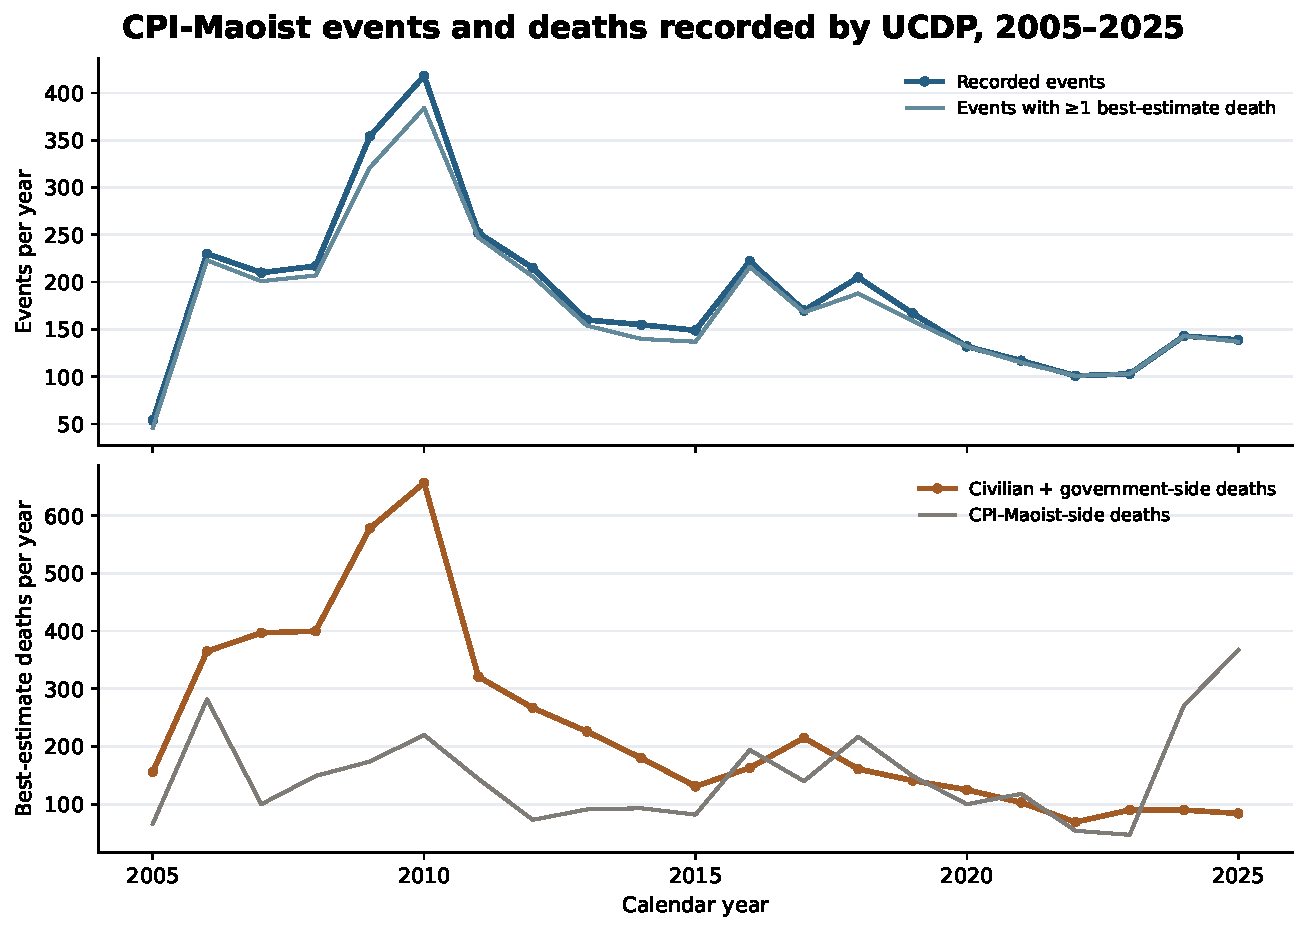
\includegraphics[width=.92\linewidth]{../outputs/annual_activity_2005_2025.pdf}
\caption{Annual UCDP event and death counts for actor ID 195 in India. The fatal-event series requires at least one best-estimate death; the main recorded-event series does not.}
\end{figure}

\clearpage
\begin{landscape}
\begin{figure}[p]
\centering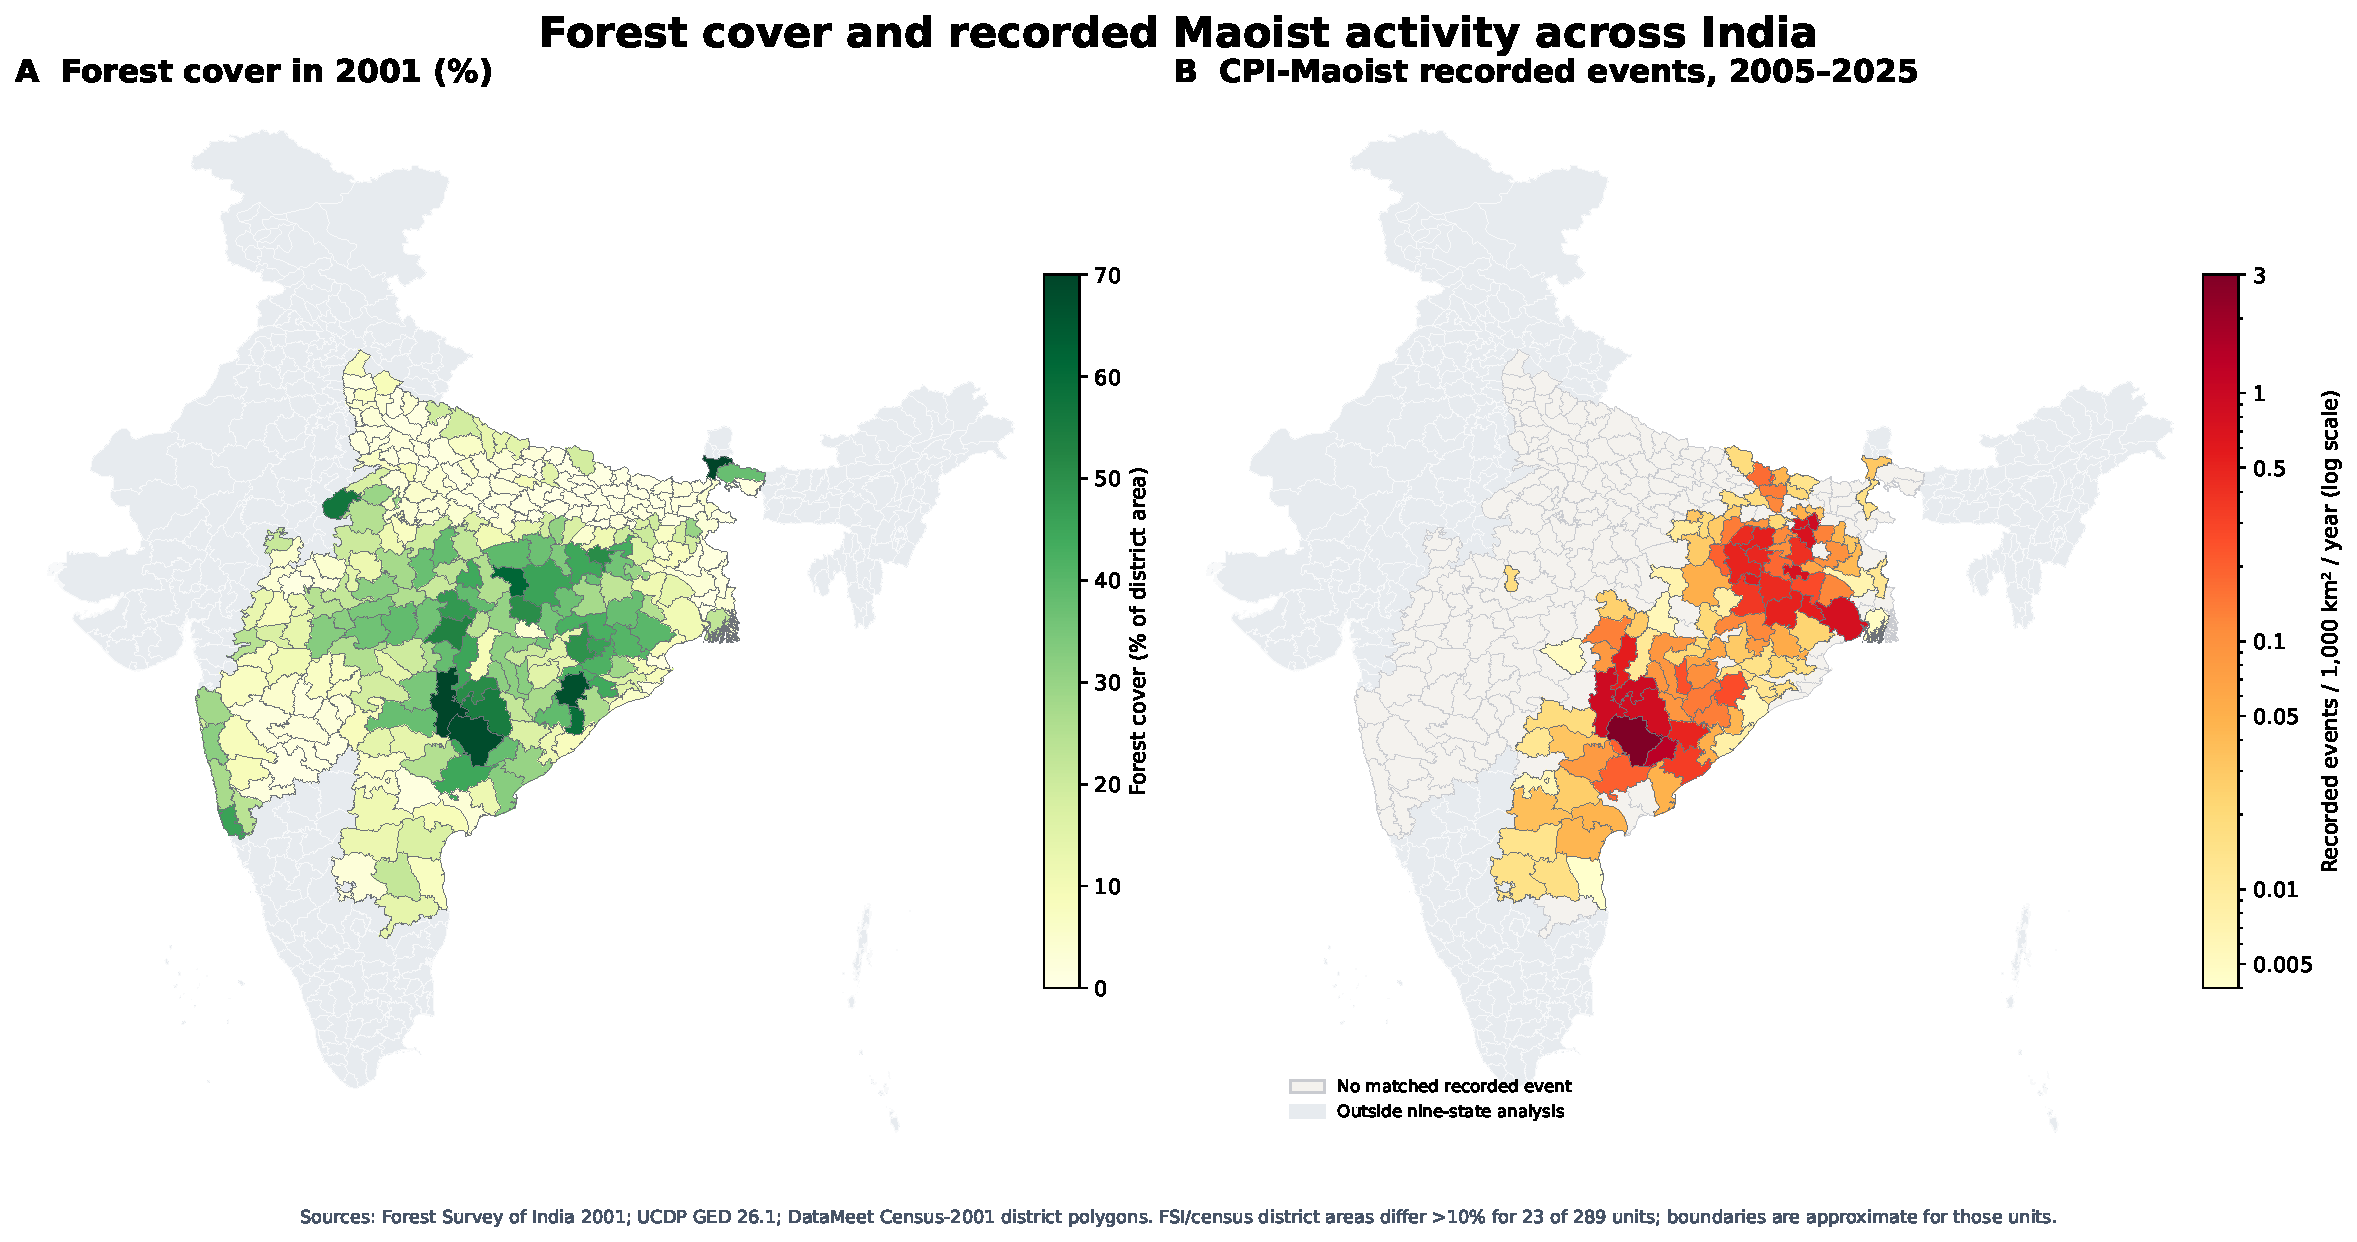
\includegraphics[width=.97\linewidth]{../outputs/india_forest_activity_maps.pdf}
\caption{District-level thematic maps on DataMeet Census 2001 polygons. Left: FSI 2001 forest-cover share. Right: UCDP recorded-event rate per 1,000 km$^2$ per year, 2005--2025; positive rates use a logarithmic colour scale. Pale gray districts are outside the nine-state analysis. Census/FSI district areas differ by over 10\% for 23 units, so the district geography is approximate there. These are aggregated maps, not event-site locations.}
\label{fig:maps}
\end{figure}
\end{landscape}
\clearpage

\begin{landscape}
\begin{figure}[p]
\centering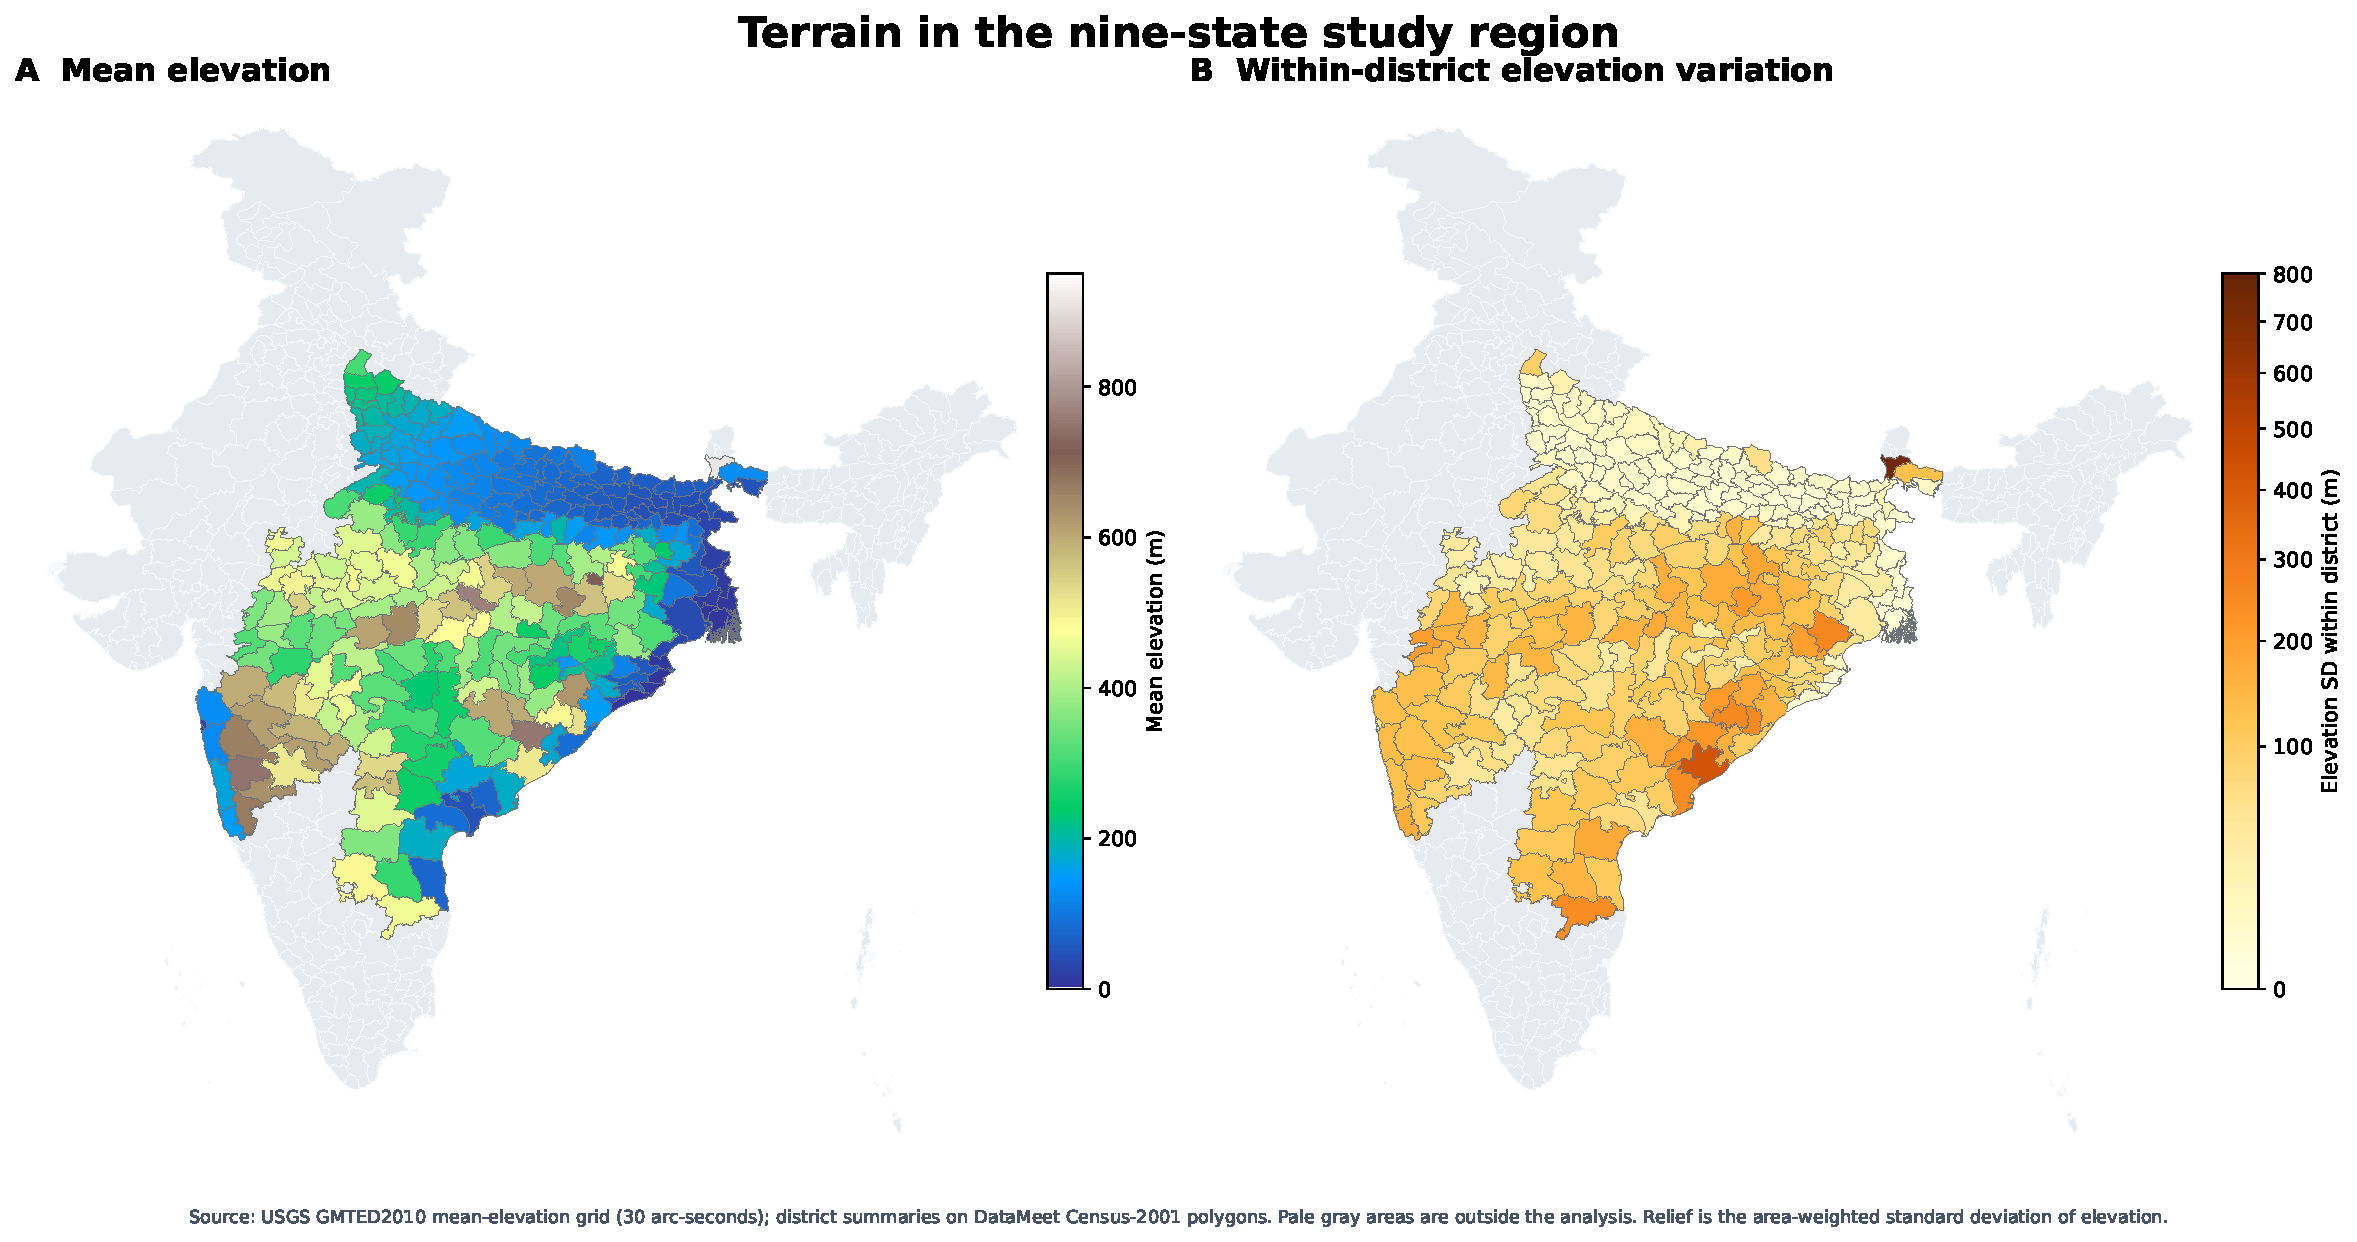
\includegraphics[width=.97\linewidth]{../outputs/india_terrain_maps.pdf}
\caption{GMTED2010 terrain summaries on the approximate Census 2001 district geography. Left: mean elevation. Right: within-district elevation SD, the relief control used in regression. The grid is 30 arc-seconds and the district summaries use cosine-latitude area weights. The area-discrepancy caveat in Figure~\ref{fig:maps} applies here too.}
\label{fig:terrain-maps}
\end{figure}
\end{landscape}
\clearpage

\section{Regression specifications and results}
The basic model is a Poisson pseudo-maximum-likelihood count regression,
\[
\log E[Y_i]=\log(21A_i/1000)+\alpha_{s(i)}+\beta F_i/10,
\]
where $Y_i$ is the 21-year event count, $A_i$ the published FSI area in km$^2$, $\alpha_{s(i)}$ a 2001-state indicator, and $F_i$ forest-cover percentage. Exponentiating $\beta$ gives an event-rate ratio for 10 percentage points more forest within a state. District-robust sandwich intervals account for overdispersion at the district level. They do not handle spatial correlation between nearby districts. The Pearson dispersion of the simple Poisson fit is 27.2, and ordinary Poisson standard errors would be too small.

The demographic-adjusted Poisson adds log 2001 population density, ST and SC shares (each per 10 points), and 2001 literacy (per 10 points). The terrain-adjusted specification adds mean elevation and within-district elevation SD, each per 100 m, while retaining the log area-years offset. These are pre-period or approximately fixed district attributes; the terrain summaries are not direct measures of travel difficulty. The negative-binomial NB2 model estimates a separate overdispersion parameter. The logistic model instead asks whether a district has \emph{any} recorded event and includes log area as a covariate; its odds ratio is not an event-rate ratio.

\begin{table}[htbp]
\centering\small
\caption{Forest association across models: ratio per 10 percentage points higher 2001 cover}
\begin{tabular}{p{7.3cm}rrr}
\toprule
Model and sample & $N$ & Ratio [95\% robust interval] & $p$\\
\midrule
Poisson, area offset and state effects & 289 & 1.79 [1.42, 2.26] & $<.001$\\
Poisson, additionally log population density & 289 & 1.25 [1.00, 1.57] & .048\\
Poisson, additionally ST, SC and literacy & 289 & 1.31 [1.03, 1.65] & .026\\
Poisson, state effects and terrain only & 289 & 1.92 [1.62, 2.28] & $<.001$\\
Poisson, demographics and terrain & 289 & 1.37 [1.06, 1.76] & .015\\
Same terrain model; area discrepancy $\leq$10\% & 266 & 1.31 [1.02, 1.68] & .036\\
Same terrain model; all three areas agree $\leq$10\% & 256 & 1.31 [1.00, 1.70] & .048\\
Same terrain model; omit highest-count unit & 288 & 1.35 [1.05, 1.75] & .020\\
Same terrain model; omit Jharkhand & 271 & 1.12 [0.81, 1.55] & .502\\
NB2 count model, demographics and terrain & 289 & 2.33 [1.84, 2.93] & $<.001$\\
Logit for any event, demographics and terrain (odds ratio) & 289 & 2.56 [1.49, 4.41] & $<.001$\\
Poisson for civilian + government-side deaths, with terrain & 289 & 1.32 [1.01, 1.73] & .046\\
\bottomrule
\end{tabular}
\label{tab:models}
\end{table}

The first coefficient reproduces an independent NumPy implementation to machine precision. Demographic adjustment reduces the forest ratio from 1.79 to 1.31; adding both terrain controls raises it modestly to 1.37, rather than removing it. The terrain-adjusted ratio is 1.31 in both area-consistency checks and 1.35 without the highest-count unit. The first check limits the FSI--census area discrepancy to 10\%; the second also limits the FSI--terrain polygon discrepancy to 10\%. Yet the estimate is near one and imprecise without Jharkhand, and the leave-one-state-out estimates vary. Mean elevation and relief have conditional ratios 0.89 (0.75--1.07) and 0.94 (0.61--1.44) per 100 m in the full Poisson model; neither has a narrow interval. NB2 estimates a larger conditional forest ratio, reflecting different weighting under severe overdispersion. A quadratic forest term did not show clear curvature in the terrain-adjusted robust coefficient test ($p=.43$); this is not evidence that the true relationship is linear. Full terrain-adjusted coefficient estimates and model metadata are in the machine-readable project files.

\begin{figure}[htbp]
\centering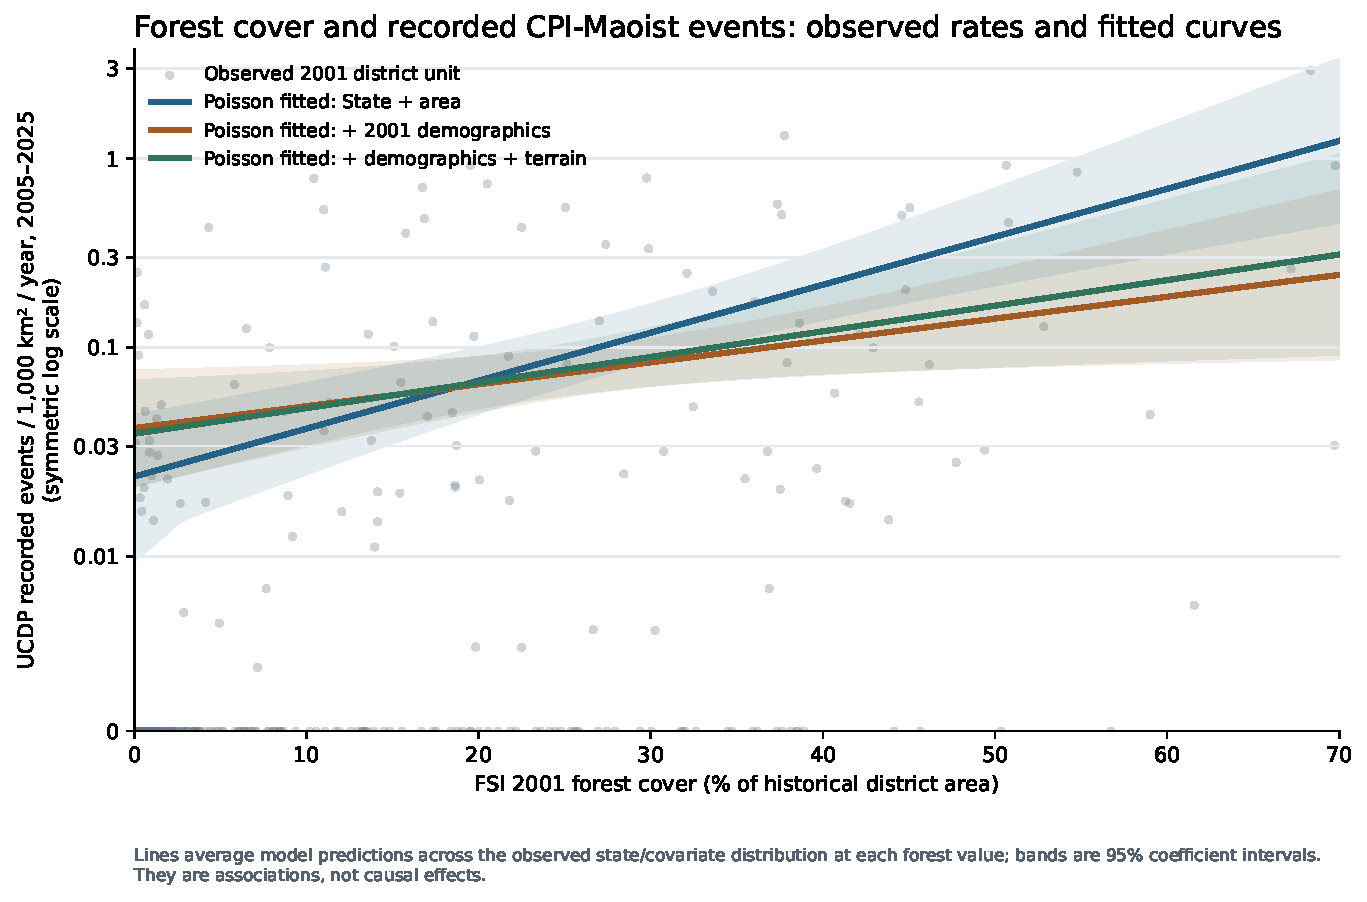
\includegraphics[width=.96\linewidth]{../outputs/forest_regression_fitted_curves.pdf}
\caption{Observed district event rates and fitted regression curves from three Poisson specifications. At each forest value, predictions are averaged across the observed state and baseline-covariate distribution; the shaded bands are 95\% district-robust coefficient intervals. This standardization can create uncommon covariate combinations, especially at the extremes. The vertical axis uses a symmetric logarithmic scale to show zero-event districts and high-rate districts together.}
\label{fig:regression-curves}
\end{figure}

Figure~\ref{fig:regression-curves} makes the fitted relationships visible on the outcome scale. At 10\% forest cover, standardized predicted rates are 0.037 for the state-only model, 0.049 with demographics, and 0.048 with demographics and terrain. At 40\%, they are 0.215, 0.109, and 0.122 events per 1,000 km$^2$ per year. The adjusted slopes are flatter than the state-only slope because the additional variables absorb part of the association. These fitted curves are descriptive model predictions, not a change in violence expected from altering a district's forests.

\begin{figure}[htbp]
\centering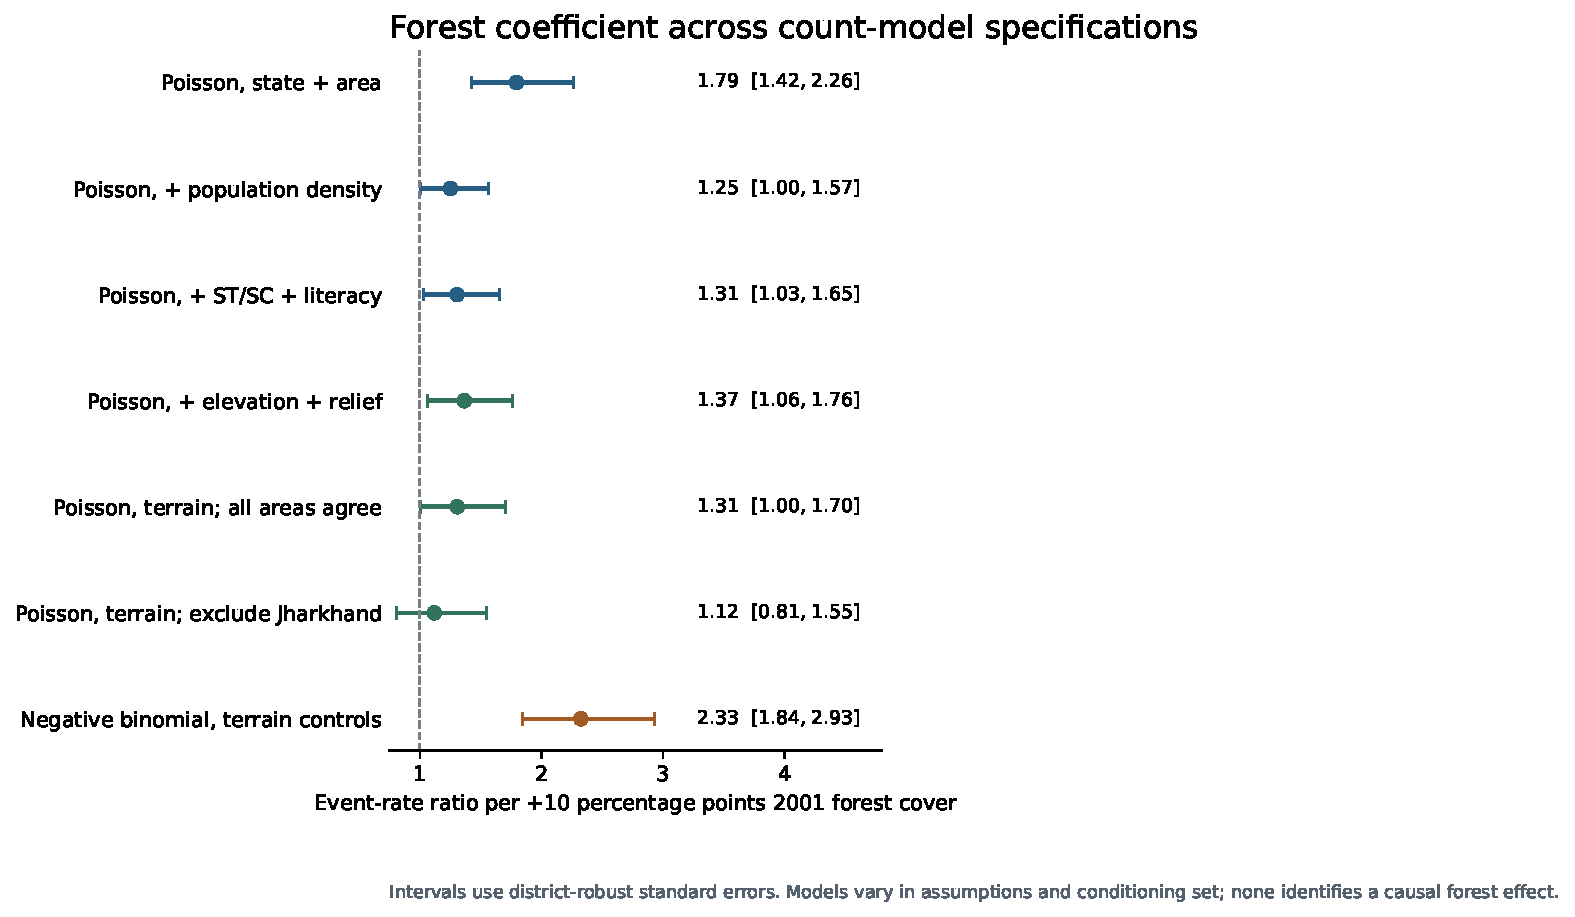
\includegraphics[width=.96\linewidth]{../outputs/model_comparison.pdf}
\caption{Count-model forest coefficients and district-robust intervals. The plotted models have different controls, samples, and variance assumptions; comparing them tests sensitivity, not causality.}
\end{figure}

\section{Exploratory baseline profiles: PCA and clustering}
To examine how forest cover co-occurs with other pre-period district traits, five baseline variables were standardized: forest-cover percentage, ST share, SC share, literacy, and log population density. No violence measure entered PCA or clustering. Principal component 1 explains 49.6\% of baseline-feature variance; its largest loadings are forest cover $+0.54$, ST share $+0.57$, log density $-0.50$, and SC share $-0.37$. Principal component 2 explains 20.4\% and is dominated by literacy ($+0.98$). These are mathematical summaries of correlated baseline variables, not mechanisms.

K-means with $k=2$ had the highest silhouette among $k=2,\ldots,6$ (0.35, indicating only moderate separation). The 90-unit higher-forest cluster averages 34.3\% forest and 31.7\% ST share, versus 7.1\% and 3.0\% in the 199-unit other cluster. Its pooled raw recorded-event rate is 0.209 rather than 0.035 per 1,000 km$^2$ per year. Since forest itself is a cluster feature and the clusters mix states, the activity contrast is descriptive only. The clustering mainly reinforces how difficult it is to isolate forest from broader demographic and settlement geography.

\begin{figure}[htbp]
\centering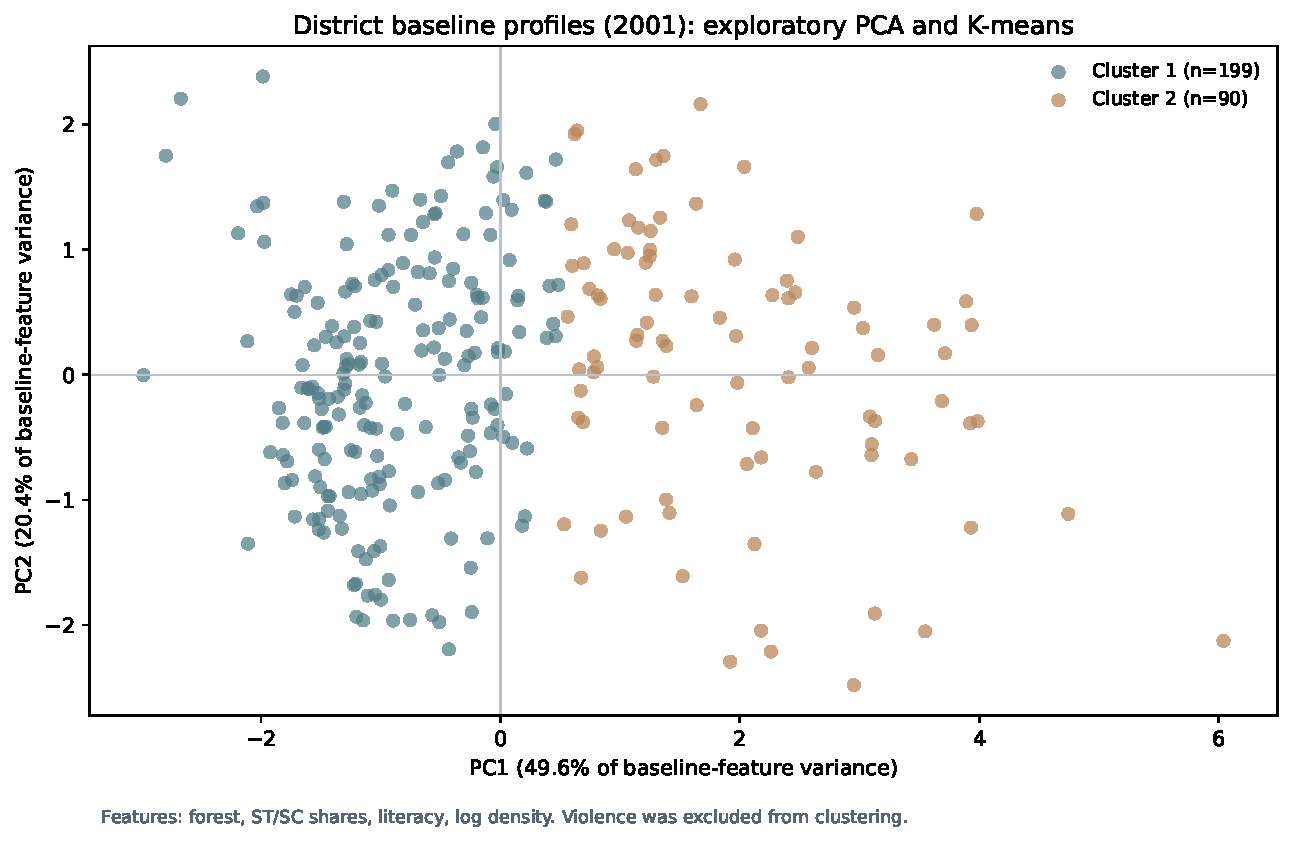
\includegraphics[width=.82\linewidth]{../outputs/pca_clusters.pdf}
\caption{PCA projection and K-means grouping using only baseline 2001 variables. Violence was excluded from the feature set.}
\end{figure}

\section{Interpretation, limits, and next research step}
The maps and regressions agree that recorded activity is concentrated in parts of the forested central and eastern belt. They do not imply that increasing forest cover would raise violence. Forests may proxy isolation, road access, state capacity, mining, land rights, pre-existing networks, and reporting conditions. Measured elevation and district-scale relief are now included, but they cannot capture all physical accessibility. Area and state controls alone leave a large positive association; adding population and social covariates reduces it; adding terrain changes it modestly; leave-one-state-out results still widen uncertainty about its magnitude.

Further limitations matter: UCDP actor ID 195 does not measure all Naxal organizations or nonfatal activity; source reporting can vary by accessibility; 150 event records are unmatched; some historical district assignments simplify changed boundaries; and the nine-state sample is geographically selected. Forest cover is fixed at 2001, while violence spans 21 years. The relief statistic can vary with district size and shape, and the two terrain controls share Census 2001 polygon discrepancies with the maps. District-level confidence intervals assume independent district scores and may be optimistic under spatial dependence. PCA and clusters are exploratory and do not improve identification.

A next stage should obtain a consistent 2001 forest raster and time-stable district or grid boundaries, pre-2005 road access, and spatially robust uncertainty estimates. If the project aims to make a causal statement, it needs a separate design based on plausibly exogenous variation. The present analysis answers the narrower question: forest cover is associated with later recorded CPI-Maoist activity in these districts, even after these terrain summaries are included, but the adjusted magnitude and mechanism remain unresolved.

\section{Additional data sources reviewed}
Several newly checked sources could strengthen a follow-up analysis. The University of Maryland's \href{https://storage.googleapis.com/earthenginepartners-hansen/GFC-2025-v1.13/download.html}{Global Forest Change v1.13} provides 30-m tree-canopy cover for 2000 and annual tree-cover loss through 2025. It is a useful alternative baseline forest measure and a possible time-varying descriptive series, but canopy cover is not FSI forest cover, and the producer cautions against naive comparison of annual loss across sensor and algorithm changes. The \href{https://www.mha.gov.in/en/documents/annual-reports}{Indian Ministry of Home Affairs annual reports} contain LWE incident and death counts that could validate broad temporal patterns; their definition of LWE incidents differs from the actor-specific UCDP outcome. The European Commission's \href{https://human-settlement.emergency.copernicus.eu/ghs_buS2023.php}{Global Human Settlement Layer} has a 2000 built-up-surface grid that could improve pre-period settlement controls. \href{https://acleddata.com/methodology/countrytime-period-coverage}{ACLED} covers India from 2016, so it could provide a later-period event robustness check but cannot reproduce the full 2005--2025 outcome. These sources have been reviewed, not silently merged into the present model; the project records their uses and limits.

\section*{Data and reproducibility}
The accompanying GitHub-ready project includes source snapshots, explicit 2001 crosswalks, the derived terrain table, intermediate analysis panels, model output CSVs, figures, scripts, a dependency file, and a reproduction guide. The event extract is reproducible from the UCDP India subset and actor file. FSI tables are extracted from the official PDF and checked against published state totals. The large public-domain USGS terrain archive is fetched by an optional hash-checked script, then district controls are regenerated. Shapes are supplied under DataMeet's CC BY 4.0 licence. The source-file hashes and exact commands are in the project README.

\begin{thebibliography}{9}
\bibitem{FSI} Forest Survey of India. \emph{State of Forest Report 2001}. \href{https://fsi.nic.in/documents/sfr_2001_hindi.pdf}{Official report}.
\bibitem{UCDP} Uppsala Conflict Data Program. \emph{Georeferenced Event Dataset, version 26.1}. \href{https://ucdp.uu.se/downloads/}{Download centre and codebook}. See also Davies, Pettersson, and \"Oberg (2026), \emph{Journal of Peace Research}, \href{https://doi.org/10.1093/jopres/xjag046}{doi:10.1093/jopres/xjag046}; and Sundberg and Melander (2013), \emph{Journal of Peace Research} 50(4).
\bibitem{WB} World Bank. \emph{India Spatial Database, Level 2, 2001}. \href{https://datacatalog.worldbank.org/search/dataset/0062657/india-spatial-database}{Data catalogue}.
\bibitem{Geometry} DataMeet. \emph{Census 2001 India district boundaries}, mirrored by \href{https://github.com/yashveeeeeeer/india-geodata/tree/main/data/administrative/districts/census-2001}{India Geodata}. CC BY 4.0.
\bibitem{Terrain} USGS and NGA. \emph{Global Multi-resolution Terrain Elevation Data 2010}, 30-arc-second mean-elevation grid. \href{https://topotools.cr.usgs.gov/gmted_viewer/gmted2010_global_grids.php}{Official download page}. Public domain.
\end{thebibliography}
\end{document}
